\section{Experiments and Observations}
\label{sec:exp}

All numbers below are generated from the recorded result files by one exporter script
(Appendix~\ref{app:repro}). Table~\ref{tab:stage1} in the appendix lists all stage-1 methods,
including the weight-space baselines, which are not discussed further here.

\subsection{The original observation and what its numbers compare}
\label{sec:orig}

\begin{table}[t]
\caption{The original calibration draw of each teacher, stage 1 and stage 2. Each column is one
teacher. The same fitted matrix is evaluated three ways: the test sample (seen during development),
the exact population objective $F$, and the calibration objective $\Fhat$ it was fitted on. The
stage-1 and stage-2 fits are bit-identical (matching SHA-256 of the merged matrices).}
\label{tab:orig}
\centering\small
% AUTO-GENERATED
\begin{tabular}{llccc}
\toprule
Solution & Evaluation & Teacher 0 & Teacher 1 & Teacher 2 \\
\midrule
Minimax & test sample ($n{=}512$, seen) & 0.713 & 0.802 & 1.057 \\
Minimax & population $F$ & 0.726 & 0.768 & 1.081 \\
Minimax & calibration $\hat F$ & 0.449 & 0.463 & 0.503 \\
Uniform WRRR & test sample ($n{=}512$, seen) & 0.642 & 0.660 & 0.754 \\
Uniform WRRR & population $F$ & 0.657 & 0.655 & 0.780 \\
Uniform WRRR & calibration $\hat F$ & 0.536 & 0.624 & 0.643 \\
\bottomrule
\end{tabular}

\end{table}

Stage~1 reported mean test worst-task errors of \SOneMinimaxTestWorstMean{} for minimax and
\SOneUniformTestWorstMean{} for uniform WRRR. Table~\ref{tab:orig} separates the comparisons that
were later conflated in a summary. The triple \SOneMinimaxTestWorstSeedA/\SOneMinimaxTestWorstSeedB/%
\SOneMinimaxTestWorstSeedC{} is the \emph{minimax} solution on the \emph{test sample}. The triple
\STwoOrigMinimaxPopTA/\STwoOrigMinimaxPopTB/\STwoOrigMinimaxPopTC{} is the \emph{same} solution
under the \emph{population} objective. Sample and population agree closely, so the original gap is
not an artefact of the test sample. On this draw the minimax solution is worse than the uniform
solution for every teacher under both evaluations. It is also the solution with the lowest
calibration objective in every column; for minimax the calibration errors of all tasks are
equalised at the value shown in the ``calibration $\Fhat$'' row.

\subsection{Is the optimiser the problem?}

\begin{table}[t]
\caption{Numerical audit of the \STwoNFits{} minimax fits in stage~2, by arm. The relative gap is
$(\mathrm{UB}-\mathrm{LB})/\mathrm{UB}$ on the fitted objective. The second column of numbers
compares the lower bound with an independent reduced-rank regression computed from raw samples at
the same $\lambda^\star$. The last three columns are the smallest task weight, the largest
condition number of $A_{\lambda^\star}$, and the smallest relative singular-value gap at the
truncation boundary. Floating-point values, not certificates.}
\label{tab:audit}
\centering\small
\resizebox{\linewidth}{!}{% AUTO-GENERATED
\begin{tabular}{lcccccc}
\toprule
Moment / normaliser & Fits & max rel.\ gap & max $|g-g_{\mathrm{ref}}|/g_{\mathrm{ref}}$ & min $\lambda_k$ & max $\kappa(S_\lambda)$ & min $(\sigma_r-\sigma_{r+1})/\sigma_r$ \\
\midrule
Emp/Emp & 12 & $7.4\times10^{-10}$ & $2.5\times10^{-15}$ & 0.136 & 19.3 & 0.109 \\
Emp/Pop & 12 & $5.8\times10^{-10}$ & $2.5\times10^{-15}$ & 0.130 & 16.3 & 0.041 \\
Pop/Emp & 12 & $2.0\times10^{-9}$ & $1.3\times10^{-15}$ & 0.170 & 7.9 & 0.011 \\
Pop/Pop & 3 & $5.9\times10^{-10}$ & $1.1\times10^{-15}$ & 0.165 & 6.1 & 0.014 \\
\bottomrule
\end{tabular}
}
\end{table}

Table~\ref{tab:audit} summarises the audit.
\begin{itemize}
\item Every fit closes its dual gap to at most $\STwoMaxGapRel$ in relative terms. In
\STwoNRefined{} fits the primal refinement stage was needed.
\item The lower bounds agree with the independent raw-data reference to within $\STwoMaxGDisc$.
\item Every achieved upper bound agrees with a raw-sample re-evaluation to within $\STwoMaxUBDisc$.
\item All solutions satisfy the rank constraint: $\sigma_{r+1}/\sigma_1\le\STwoMaxRankRatio$.
\item All $\lambda^\star$ lie in the interior of the simplex (smallest weight \STwoMinLambda).
\item Each $A_{\lambda^\star}$ is well conditioned (condition number at most \STwoMaxCond).
\item The smallest relative singular-value gap at the truncation boundary is \STwoMinSvGap.
\end{itemize}
This gap is small for some Pop/Emp fits but nonzero, so by Proposition~\ref{prop:rrr} the inner
minimiser at $\lambda^\star$ is unique on every instance. On these instances a large optimisation
error therefore does not explain the calibration--population discrepancy. This rules out neither
every possible implementation bug nor failure on other problems.

\subsection{Oracle substitution: moments versus normalisers}

\begin{table}[t]
\caption{Paired difference $\Delta=F(\What_{\mathrm{minimax}})-F(\What_{\mathrm{uniform}})$ on
the population objective; negative values favour minimax. The teacher columns average the
\CfgNResamples{} fresh draws of that teacher, and the last column averages all \CfgNewCells{}
nested cells. Pop/Pop does not depend on the draw and is computed once per teacher.}
\label{tab:2x2}
\centering\small
% AUTO-GENERATED
\begin{tabular}{lcccc}
\toprule
Moment / normaliser & Teacher 0 & Teacher 1 & Teacher 2 & Mean over 9 cells (sd) \\
\midrule
Emp/Emp & $-$0.041 & $-$0.014 & +0.075 & +0.007 (0.078) \\
Emp/Pop & +0.034 & $-$0.002 & +0.086 & +0.039 (0.082) \\
Pop/Emp & $-$0.041 & $-$0.025 & $-$0.010 & $-$0.025 (0.043) \\
Pop/Pop & $-$0.066 & $-$0.137 & $-$0.076 & $-$0.093 (--) \\
\bottomrule
\end{tabular}

\end{table}

\begin{figure}[t]
\centering
% AUTO-GENERATED by paper/tools/export_results.py (TikZ; teacher means over the 3 new draws;
% Pop/Pop uses no calibration draw). Colours: validated categorical slots 1-2.
\definecolor{unifc}{HTML}{2A78D6}
\definecolor{minic}{HTML}{EB6834}
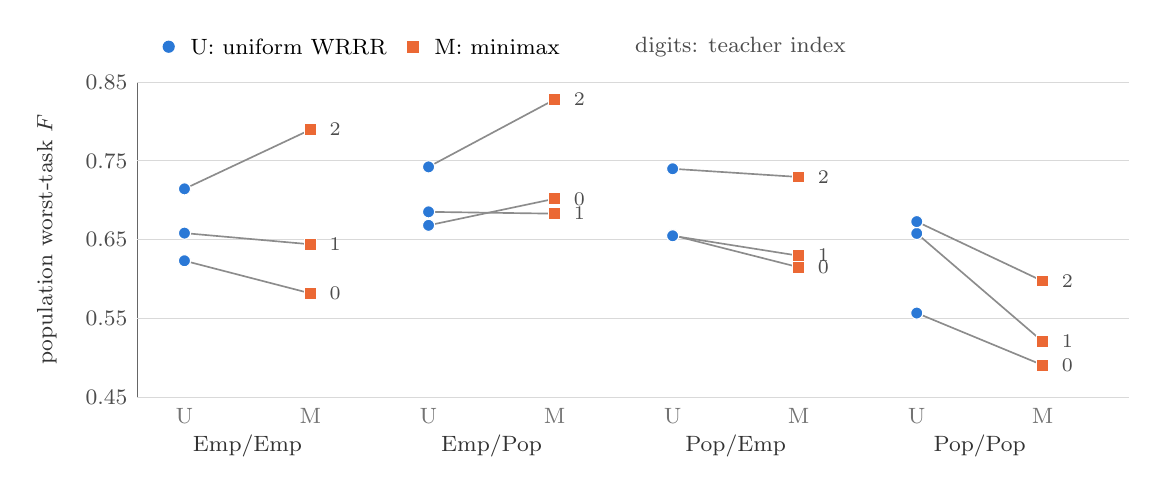
\begin{tikzpicture}[x=1cm,y=1cm,font=\footnotesize]
\draw[black!60] (0,0) -- (0,4.000);
\draw[black!15] (0,0.000) -- (12.6,0.000);
\node[anchor=east,text=black!70] at (0,0.000) {0.45};
\draw[black!15] (0,1.000) -- (12.6,1.000);
\node[anchor=east,text=black!70] at (0,1.000) {0.55};
\draw[black!15] (0,2.000) -- (12.6,2.000);
\node[anchor=east,text=black!70] at (0,2.000) {0.65};
\draw[black!15] (0,3.000) -- (12.6,3.000);
\node[anchor=east,text=black!70] at (0,3.000) {0.75};
\draw[black!15] (0,4.000) -- (12.6,4.000);
\node[anchor=east,text=black!70] at (0,4.000) {0.85};
\node[rotate=90,anchor=south,text=black!80] at (-0.9,2.000) {population worst-task $F$};
\node[anchor=north,text=black!80] at (1.40,-0.35) {Emp/Emp};
\node[anchor=north,text=black!55] at (0.60,-0.02) {U};
\node[anchor=north,text=black!55] at (2.20,-0.02) {M};
\draw[black!45,line width=0.6pt] (0.60,1.732) -- (2.20,1.318);
\fill[unifc,draw=white,line width=0.4pt] (0.60,1.732) circle (2.2pt);
\fill[minic,draw=white,line width=0.4pt] (2.125,1.243) rectangle (2.275,1.393);
\node[anchor=west,text=black!70,font=\scriptsize] at (2.32,1.318) {0};
\draw[black!45,line width=0.6pt] (0.60,2.083) -- (2.20,1.941);
\fill[unifc,draw=white,line width=0.4pt] (0.60,2.083) circle (2.2pt);
\fill[minic,draw=white,line width=0.4pt] (2.125,1.866) rectangle (2.275,2.016);
\node[anchor=west,text=black!70,font=\scriptsize] at (2.32,1.941) {1};
\draw[black!45,line width=0.6pt] (0.60,2.645) -- (2.20,3.397);
\fill[unifc,draw=white,line width=0.4pt] (0.60,2.645) circle (2.2pt);
\fill[minic,draw=white,line width=0.4pt] (2.125,3.322) rectangle (2.275,3.472);
\node[anchor=west,text=black!70,font=\scriptsize] at (2.32,3.397) {2};
\node[anchor=north,text=black!80] at (4.50,-0.35) {Emp/Pop};
\node[anchor=north,text=black!55] at (3.70,-0.02) {U};
\node[anchor=north,text=black!55] at (5.30,-0.02) {M};
\draw[black!45,line width=0.6pt] (3.70,2.182) -- (5.30,2.519);
\fill[unifc,draw=white,line width=0.4pt] (3.70,2.182) circle (2.2pt);
\fill[minic,draw=white,line width=0.4pt] (5.225,2.444) rectangle (5.375,2.594);
\node[anchor=west,text=black!70,font=\scriptsize] at (5.42,2.519) {0};
\draw[black!45,line width=0.6pt] (3.70,2.353) -- (5.30,2.330);
\fill[unifc,draw=white,line width=0.4pt] (3.70,2.353) circle (2.2pt);
\fill[minic,draw=white,line width=0.4pt] (5.225,2.255) rectangle (5.375,2.405);
\node[anchor=west,text=black!70,font=\scriptsize] at (5.42,2.330) {1};
\draw[black!45,line width=0.6pt] (3.70,2.924) -- (5.30,3.779);
\fill[unifc,draw=white,line width=0.4pt] (3.70,2.924) circle (2.2pt);
\fill[minic,draw=white,line width=0.4pt] (5.225,3.704) rectangle (5.375,3.854);
\node[anchor=west,text=black!70,font=\scriptsize] at (5.42,3.779) {2};
\node[anchor=north,text=black!80] at (7.60,-0.35) {Pop/Emp};
\node[anchor=north,text=black!55] at (6.80,-0.02) {U};
\node[anchor=north,text=black!55] at (8.40,-0.02) {M};
\draw[black!45,line width=0.6pt] (6.80,2.056) -- (8.40,1.650);
\fill[unifc,draw=white,line width=0.4pt] (6.80,2.056) circle (2.2pt);
\fill[minic,draw=white,line width=0.4pt] (8.325,1.575) rectangle (8.475,1.725);
\node[anchor=west,text=black!70,font=\scriptsize] at (8.52,1.650) {0};
\draw[black!45,line width=0.6pt] (6.80,2.049) -- (8.40,1.796);
\fill[unifc,draw=white,line width=0.4pt] (6.80,2.049) circle (2.2pt);
\fill[minic,draw=white,line width=0.4pt] (8.325,1.721) rectangle (8.475,1.871);
\node[anchor=west,text=black!70,font=\scriptsize] at (8.52,1.796) {1};
\draw[black!45,line width=0.6pt] (6.80,2.900) -- (8.40,2.796);
\fill[unifc,draw=white,line width=0.4pt] (6.80,2.900) circle (2.2pt);
\fill[minic,draw=white,line width=0.4pt] (8.325,2.721) rectangle (8.475,2.871);
\node[anchor=west,text=black!70,font=\scriptsize] at (8.52,2.796) {2};
\node[anchor=north,text=black!80] at (10.70,-0.35) {Pop/Pop};
\node[anchor=north,text=black!55] at (9.90,-0.02) {U};
\node[anchor=north,text=black!55] at (11.50,-0.02) {M};
\draw[black!45,line width=0.6pt] (9.90,1.068) -- (11.50,0.406);
\fill[unifc,draw=white,line width=0.4pt] (9.90,1.068) circle (2.2pt);
\fill[minic,draw=white,line width=0.4pt] (11.425,0.331) rectangle (11.575,0.481);
\node[anchor=west,text=black!70,font=\scriptsize] at (11.62,0.406) {0};
\draw[black!45,line width=0.6pt] (9.90,2.079) -- (11.50,0.705);
\fill[unifc,draw=white,line width=0.4pt] (9.90,2.079) circle (2.2pt);
\fill[minic,draw=white,line width=0.4pt] (11.425,0.630) rectangle (11.575,0.780);
\node[anchor=west,text=black!70,font=\scriptsize] at (11.62,0.705) {1};
\draw[black!45,line width=0.6pt] (9.90,2.229) -- (11.50,1.473);
\fill[unifc,draw=white,line width=0.4pt] (9.90,2.229) circle (2.2pt);
\fill[minic,draw=white,line width=0.4pt] (11.425,1.398) rectangle (11.575,1.548);
\node[anchor=west,text=black!70,font=\scriptsize] at (11.62,1.473) {2};
\fill[unifc] (0.4,4.450) circle (2.2pt);
\node[anchor=west] at (0.55,4.450) {U: uniform WRRR};
\fill[minic] (3.425,4.375) rectangle (3.575,4.525);
\node[anchor=west] at (3.65,4.450) {M: minimax};
\node[anchor=west,text=black!70] at (6.2,4.450) {digits: teacher index};
\end{tikzpicture}

\caption{Teacher-level paired comparison on the population worst-task error $F$. For each arm,
the U (uniform WRRR, circle) and M (minimax, square) values of each teacher are joined by a line,
using means over the \CfgNResamples{} fresh draws (Pop/Pop does not depend on the draw).
Lower is better. Per-draw values are in
Table~\ref{tab:perdraw}.}
\label{fig:paired}
\end{figure}

Table~\ref{tab:2x2} and Figure~\ref{fig:paired} give the four arms. The pre-registered verdicts
are:
\begin{itemize}
\item Emp/Emp: \STwoVerdictEE{} (mean $\Delta$ \STwoDeltaEE, sd over cells \STwoDeltaSDEE);
\item Emp/Pop: \STwoVerdictEP{} (\STwoDeltaEP);
\item Pop/Emp: \STwoVerdictPE{} (\STwoDeltaPE);
\item Pop/Pop: \STwoVerdictPP{} (\STwoDeltaPP).
\end{itemize}
Three observations follow.

First, the large disadvantage seen on the original draw does not reproduce on average over fresh
draws. The original draw gave \STwoOrigDeltaEETA, \STwoOrigDeltaEETB{} and \STwoOrigDeltaEETC{}
for teachers 0, 1 and 2. The fresh draws give teacher means \STwoDeltaEETA, \STwoDeltaEETB{} and
\STwoDeltaEETC. The draw-to-draw spread is of the same order as the effect.

Second, substituting population moments makes minimax better than uniform on average for both
choices of normaliser. Substituting population normalisers alone does not: Emp/Pop is worse than
Emp/Emp. One explanation we have \emph{not} tested is that, when both come from the same draw, the
moment error and the normaliser error partly cancel in the ratio.

Third, in the Pop/Pop arm the fitted objective \emph{is} the evaluation objective. That minimax
wins there (for teachers 0, 1 and 2, $F$ is \STwoPPMinimaxTA, \STwoPPMinimaxTB{} and
\STwoPPMinimaxTC{} against \STwoPPUniformTA, \STwoPPUniformTB{} and \STwoPPUniformTC) is a
consequence of optimising the right objective. It is not evidence that minimax generalises. It
does show that the evaluator and the fitted objective are consistent.

The pattern is consistent with moment-estimation noise driving the calibration--population
discrepancy. The pre-registered attribution rule, however, required the problem to be
\emph{present} in both empirical-moment arms, and Emp/Emp is ambiguous. The formal outcome is
therefore \textbf{cause undetermined}. We report the moment-noise reading as a hypothesis
supported by the oracle substitution, not as an established cause.

\subsection{Calibration optimism is distinct from the numerical gap}

\begin{table}[t]
\caption{Fitted objective of the returned solution against its population value, averaged over
the \CfgNewCells{} fresh cells. This is a statistical optimism gap. It is unrelated to the
numerical UB--LB gap of Table~\ref{tab:audit}, which is at most $\STwoMaxGapRel$ in relative terms.}
\label{tab:optimism}
\centering\small
% AUTO-GENERATED
\begin{tabular}{llccc}
\toprule
Moment / normaliser & Solution & Fitted objective $\hat F(\hat W)$ & Population $F(\hat W)$ & Difference \\
\midrule
Emp/Emp & Uniform WRRR & 0.606 & 0.665 & +0.060 \\
Emp/Emp & Minimax & 0.497 & 0.672 & +0.175 \\
Emp/Pop & Uniform WRRR & 0.622 & 0.699 & +0.076 \\
Emp/Pop & Minimax & 0.517 & 0.738 & +0.220 \\
Pop/Emp & Uniform WRRR & 0.612 & 0.684 & +0.072 \\
Pop/Emp & Minimax & 0.513 & 0.658 & +0.145 \\
\bottomrule
\end{tabular}

\end{table}

Table~\ref{tab:optimism} shows that both solutions look better on calibration data than they
are, and that the minimax solution is more optimistic in every arm that uses a calibration sample.
For example, in Emp/Emp the minimax understatement is \STwoOptGapEEMinimax, against
\STwoOptGapEEUniform{} for uniform. This fits the familiar picture that minimising a maximum of
noisy estimates selects the noise. At \CfgNcal{} samples per task the relative normaliser
estimates range from \STwoNormRatioMin{} to \STwoNormRatioMax{} times their population values.

\subsection{Do the deterministic bounds explain the gap?}
\label{sec:boundcheck}

We evaluated Corollary~\ref{cor:fixed} (Emp/Pop) and Lemmas~\ref{lem:denom} and~\ref{lem:dev}
(Emp/Emp) on all \SThreeNCells{} recorded fits. The setup was as follows:
\begin{itemize}
\item $W^\star$ is the Pop/Pop solution of the same teacher;
\item $B$ is the larger of $\fnorm{\What}$ and $\fnorm{W^\star}$, chosen after the fact, which is
legitimate because the inequalities are deterministic (median \SThreeMedianB);
\item $\epsilon_{\mathrm{opt}}$ is the fit's own UB--LB gap (at most $\SThreeMaxEps$).
\end{itemize}
The fitted matrices had been stored only as hashes. They were regenerated with the identical code
path, and all \SThreeNRefits{} regenerated matrices match their recorded SHA-256
(Appendix~\ref{app:boundcheck}).

Every inequality holds: \SThreeNBoundsHold{} of \SThreeNCells{} excess bounds and
\SThreeNPointwiseHold{} of \SThreeNPointwiseChecks{} pointwise checks of Lemmas~\ref{lem:pert}
and~\ref{lem:denom}. None of them is informative at this sample size. The relative moment error
$\max_k\opnorm{S_k-\Shat_k}/\opnorm{S_k}$ lies between \SThreeRelOpErrMin{} and
\SThreeRelOpErrMax{}. The smallest excess bound is \SThreeMinBound{} in units of relative error,
at least \SThreeMinBoundOverExcess{} times the realised excess $F(\What)-F(W^\star)$. Even the
pointwise inequalities use at most a fraction \SThreePointwiseMaxRatio{} of their right-hand side.
The bounds are therefore consistent with the observations but explain neither their size nor
their sign. With $n=\CfgNcal$ samples in dimension $q=\CfgDin$, a worst-case spectral argument is
far from tight for these fits.
